%
% Here are the many ways folks can help out.
%
% TODO I know I'm missing lots.  :-\
%

\chapter{Volunteering}
\label{ch:volunteering}

% This is true if only doing the flight manual, not the pre-flight
\ifisflight
  % This one page needs to be one column to look right, even
  % in the flight manual, proper.
  % failed experiment to add thumb guides
%   \addthumb{Welcome}{}{white}{black}
\putchapterthumb
\fi

No burn exists without volunteers and volunteers are our heroes! We have no hired help other than security and everything we do is done on a volunteer basis.  This goes for all the things before, during, and after the burn.  All the teams that you can volunteer for are described in the ``Crew Manifest'' section starting from page \pageref{ch:teams}.

There are two ways to volunteer:

\textbf{Before the event} you can sign up from the available volunteer activities by going to:

{\indent ~~~ \url{https://www.signupgenius.com/tabs/33773df01a4c3edc42-tothemoon} }

\textbf{During the event} you can go to the \gls{vc} folks at the \gls{cockpit} to sign up for an available volunteer slot.

\section*{EARLY ENTRY FOR VOLUNTEERS}
\bod[inline]{update with new early access gate hours/late checkout for volunteers if needed}

If a participant has a volunteer shift on Wednesday, they will be granted entry at noon on Wednesday.\footnote{This is mainly \gls{gate} but a few other teams have a few volunteer shift scheduled for Wednesday for set up.}  If a participant has a volunteer shift beginning before noon on Thursday they will be granted early entry on Wednesday after 3 pm.  This list will be given to \gls{gate} from \gls{vc} before \gls{gate} opens opens on Wednesday.

All participants must be off site by noon on Monday unless they have a shift on Monday after noon. In which case they will need to have permission from \gls{vc} or one of the \gls{eventleads} to stay on site for that shift, and should stop by the \gls{vc} tent on Monday before 10 am to get their approval. All late stay volunteer must also have their camp packed before their shift on Monday and be prepared to leave immediately following that last shift.\footnote{There are other early entries granted for \glspl{themecamp}, \gls{dpw}, \glspl{teamleads}, \gls{bod}, etc,,  but those lists will be given to \gls{gate} from appropriate lead for that team. This info is just for those volunteering first shifts on teams that start when gates open or before.}


% \clearpage
\section*{Volunteer Training}

\subsection*{Conclave}
We ask that all fire performers attend one of the three fire safety meetings provided by Singe City and obtain a wristband. This allows you to come spin in their fire circle each night at Headroom Village.

Fire Safety meetings will be at Singe City fire circle in Headroom Village. Spinners in Conclave must attend one of the training events listed below. You will be given a fire safe wristband to spin fire during the duration of the burn. Conclave Participants will also meet at \gls{effigyburnfield} at 2:00\pm{} Saturday afternoon, and again at 7:00\pm{} for curtain call.

\begin{center}
\footnotesize
\begin{tabular}{|c|c|c|}
\hline
\textbf{Day} & \textbf{Time} & \textbf{Place} \\ \hline
Thursday & 7\pm{} & Singe City Fire Circle\\ \hline
Friday & 7\pm{} &  Singe City Fire Circle  \\ \hline
Saturday & 2\pm{} & \gls{effigyburnfield}  \\ \hline
Saturday & 7\pm{} & \gls{effigyburnfield}  \\ \hline
\end{tabular}
\end{center}

% \clearpage

\subsection*{Perimeter}
Outer Perimeter volunteers meet at the \gls{effigyburnfield} on before the burn time and establish a burn perimeter to aid in the safety of participants during the burn. Training for these volunteers is mandatory.

Outer Perimeter meet 3\pm{} on Saturday for training, no experience needed.
Inner perimeter meet 4\pm{} on Saturday for training, must be experienced. Temple meet 3\pm{} on Sunday for training.

If you are experienced with perimeter and fire safety and want a shift doing \textbf{inner} perimeter, please email the perimeter lead directly (\url{perimeter@tothemoonburn.com}) and they will vet you for that.

\begin{center}
\footnotesize
\begin{tabular}{|c|c|c|}
\hline
\textbf{Day} & \textbf{Time} & \textbf{Place} \\ \hline
Saturday & 3\pm{} & \gls{effigyburnfield} \\ \hline
Saturday & 4\pm{} & \gls{effigyburnfield} \\ \hline
Sunday & 3\pm{} & \gls{templefield} \\ \hline
\end{tabular}
\end{center}

\subsection*{Rangers and Fire Safety}

\begin{center}
\footnotesize
\begin{tabular}{|c|c|c|}
\hline
\textbf{Day} & \textbf{Time} & \textbf{Place} \\ \hline
Thursday & 7\pm{} & \gls{moonrangerstation} \\ \hline
Friday & 1\pm{} & \gls{moonrangerstation} \\ \hline
\end{tabular}
\end{center}

\subsection*{River Safety}

Note that this safety training is open to everyone.  Anyone that wants to play in the river is strongly encouraged to attend.

\begin{center}
\footnotesize
\begin{tabular}{|c|c|c|}
\hline
\textbf{Day} & \textbf{Time} & \textbf{Place} \\ \hline
TBD & TBD & Riverfront below \gls{dpw} \\ \hline
\end{tabular}
\end{center}
\bod[inline]{will there be a river safety training?}


% \newpage
\vbox{
\subsection*{Tbase / Sanctuary}
You will also be able to sign up for volunteer shifts at the burn, at the end of the training, or you may sign up for shifts now as long as you attend a training before your shift is scheduled.

If you have volunteered for 3 or more Tranquility Base shifts in the past, please consider signing up for a shift lead slot! If you have not worked at least 3 T-base shifts, please choose a regular shift to get some more experience before signing up for Shift Lead.

\begin{center}
\footnotesize
\begin{tabular}{|c|c|c|}
\hline
\textbf{Day} & \textbf{Time} & \textbf{Place} \\ \hline
Thursday & 5\pm{} & \gls{tbass} \\ \hline
Friday & 5\pm{} & \gls{tbass} \\ \hline
\end{tabular}
\end{center}}

% \bod[inline]{add all volunteer training}
% \todo[inline]{Add information on how to volunteer before and during the event. Probably from https://www.tothemoonburn.com/volunteering}



\vspace*{\fill}
\begin{figure}[h!]
\centering
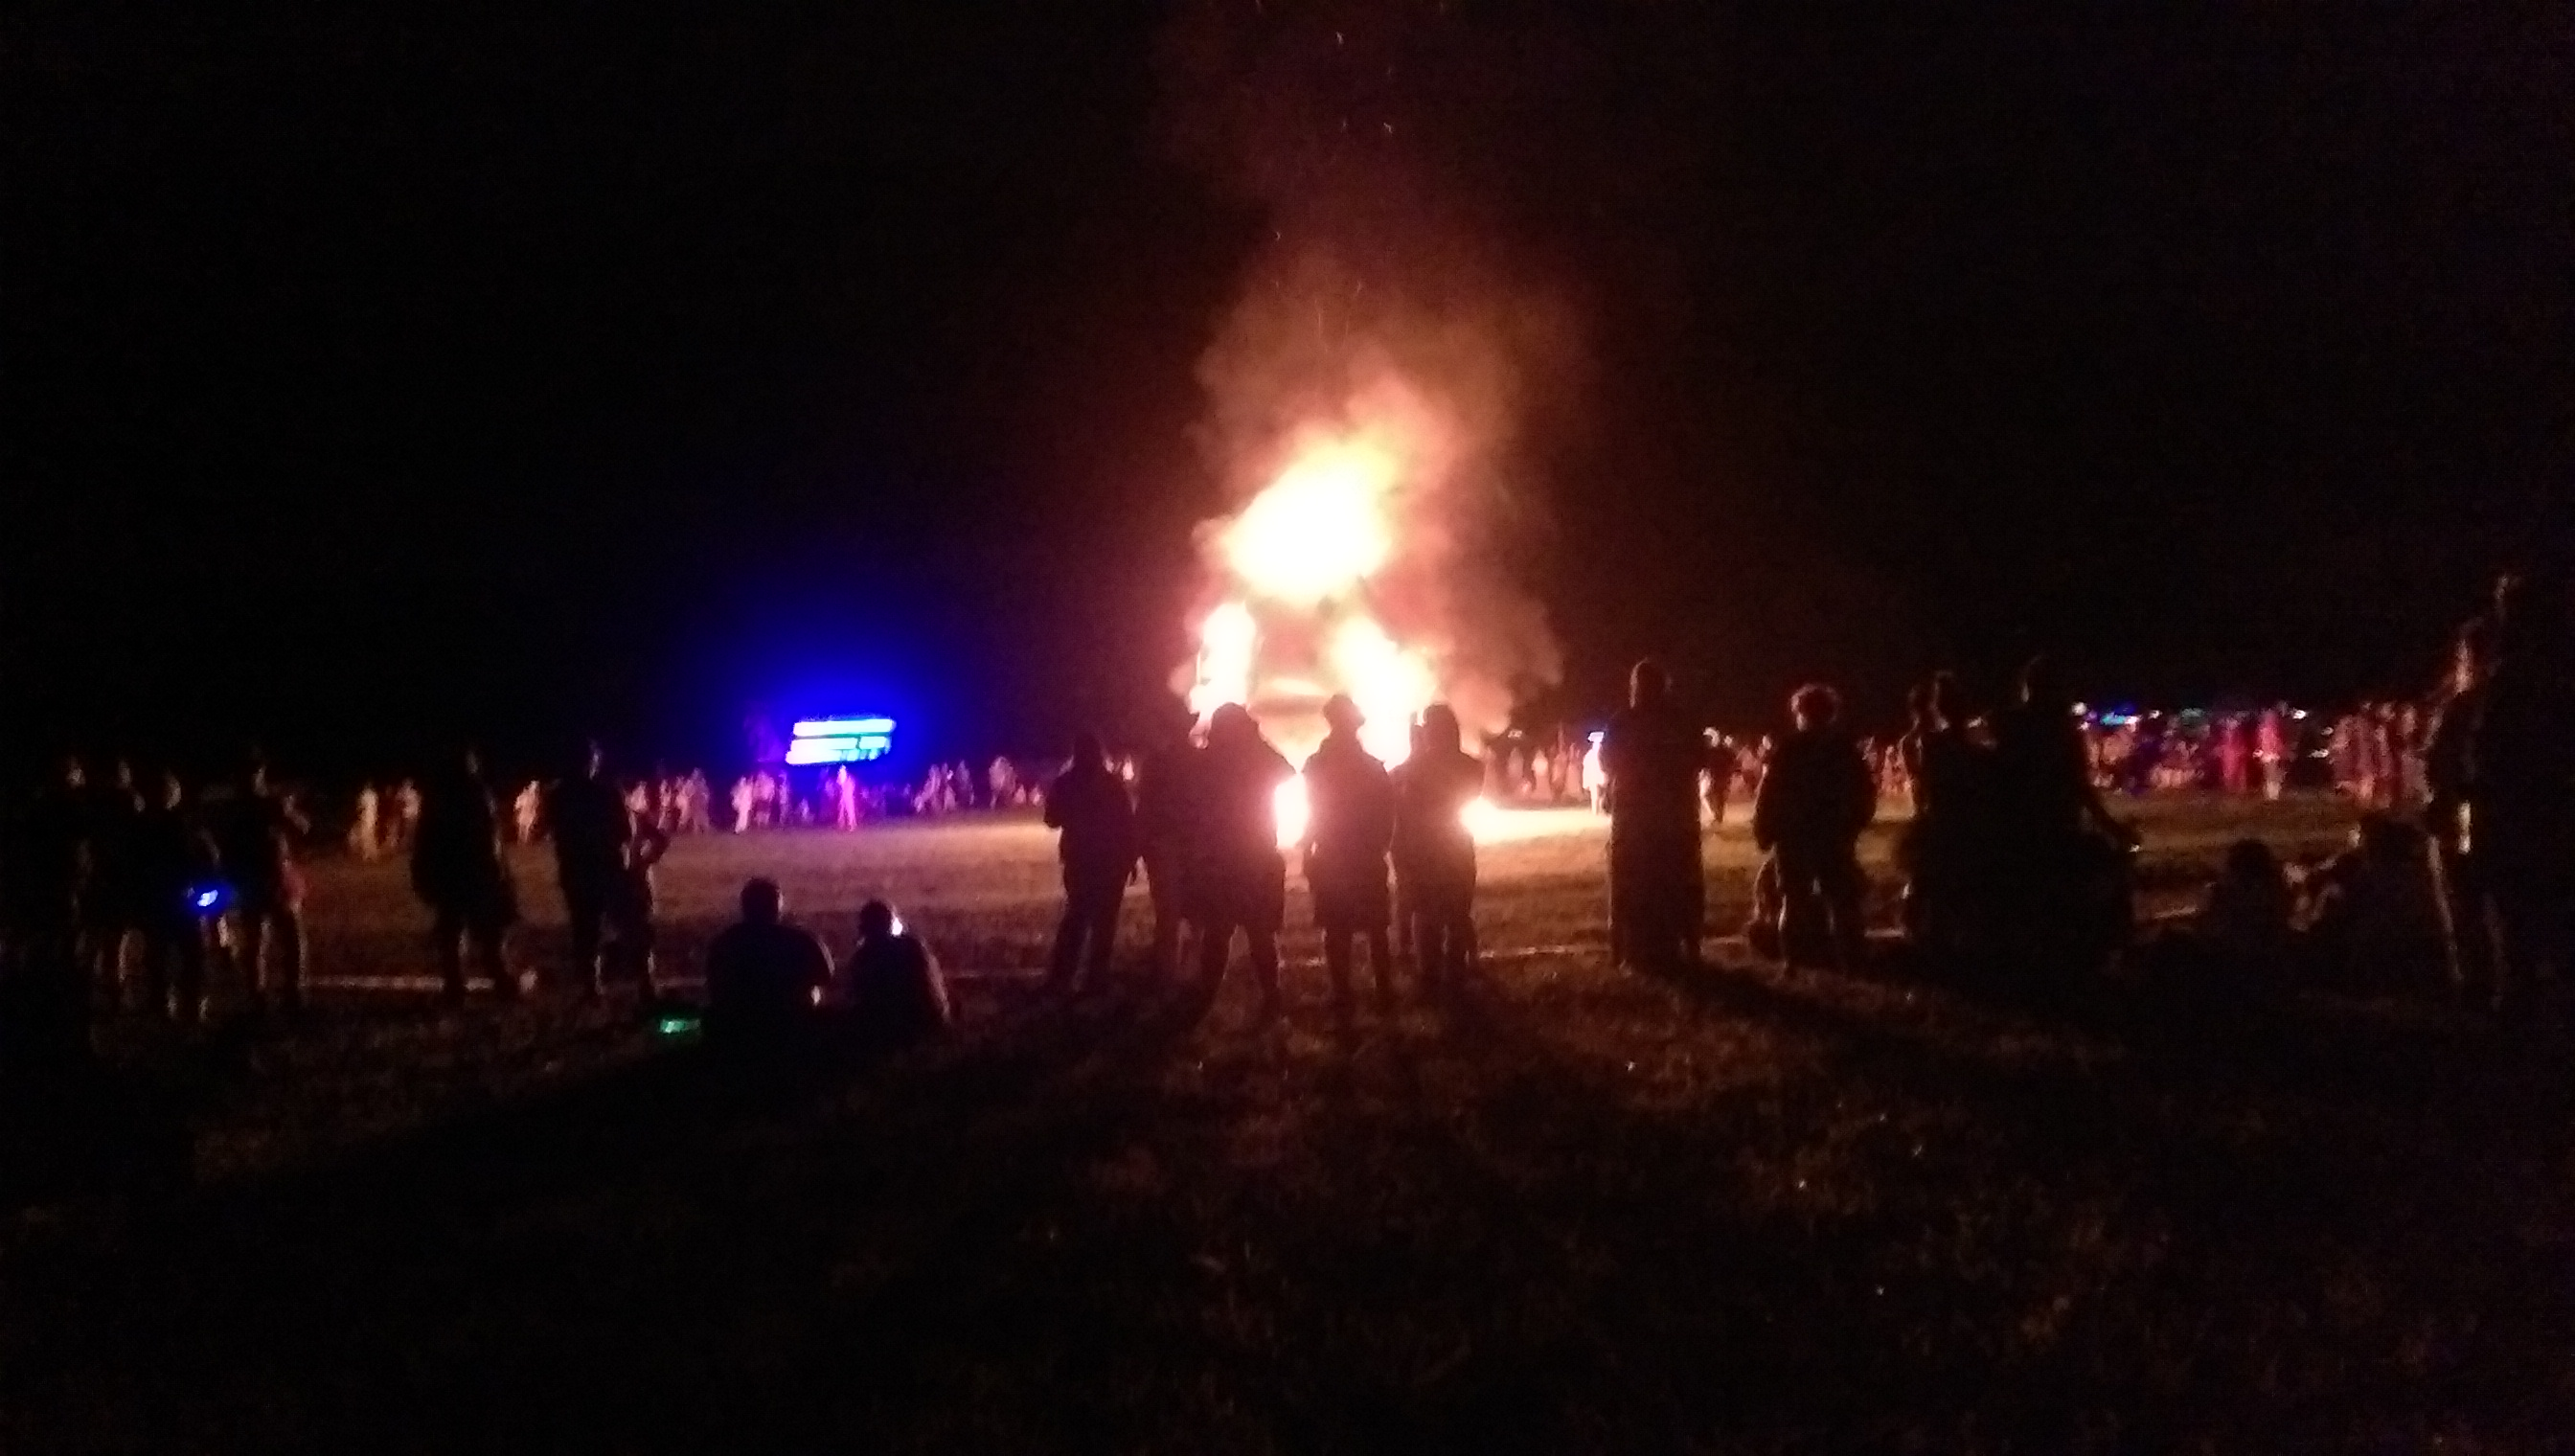
\includegraphics[width=\textwidth]{images/TTM2017EffigyBurn.jpg}
\end{figure}
\vspace*{\fill}

\newpage
\subsection*{Notes}

Note down your trainings here!


\vspace{2.5in}

\subsection*{Volunteer Shifts}

Note down you volunteer shifts here!